\documentclass[a4paper,11pt,dvipdfmx]{ujarticle}
% パッケージ
\usepackage{graphicx}
\usepackage{url}
% レイアウト指定を記述したファイルの読み込み
\input{layout}

% タイトルと氏名を変更せよ．
\title{日本におけるデジタル化の状況}
\author{G684942026 松嵜 柊}

\begin{document}

\maketitle %ここにタイトルが入る

% ここから本文
% 節見出し: \section{}
% を使う
\section{デジタル競争力ランキング}

% 本文(1)
%  参考文献の参照: \cite{}
%  図番号の参照： \ref{}
% を使う
% 文献データベースのキーワードは oecd と imd
% になっている．
国際経営開発研究所(IMD)の調査\cite{imd}によると,
日本のデジタル競争力のランキングは図\ref{fig:競争力}に示すように,
調査対象の64カ国中,総合で28位,知識分野で25位となっている.
% 図の挿入
% \includegraphics{}
% を
% \begin{figure}[htbp]
% \end{figure}
% で囲み
% \caption{}
% で図のタイトルを入れる．
% \label{}
% を使って図番号が参照できるようにする
% また，
% \centering
% で図が中央に来るようにする
\begin{figure}[htbp]
    \centering
    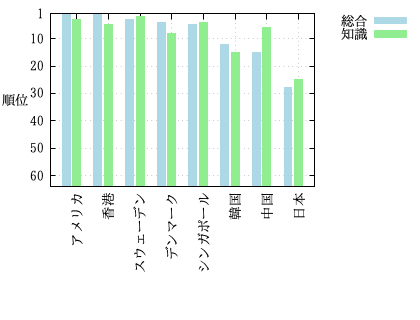
\includegraphics[width=0.7\linewidth]{fig31.png}
    \caption{デジタル競争力ランキング(64カ国中)}\label{fig:競争力}
\end{figure}
% ーーー
% 節見出し(2)
\section{ブロードバンドの整備状況}

% 本文(2)
OECDによるブロードバンド回線の普及に関する調査\cite{oecd}によると,
表\ref{fig:加入者数}に示すように,日本における100人あたりの光ファイバー回線の加入者数は29.0で,
韓国,スウェーデン,ノルウェーに続いて第4位になっている.
% 表の挿入
% \begin{tabular}
% \end{tabular}    
% による表の記述を 
% \begin{table}[htbp]
% \end{table}
% で囲み
% \caption{}
% で表のタイトルを入れる．
% \label{}
% を使って表番号が参照できるようにする
% また，
% \centering
% で表が中央に来るようにする

\begin{table}[htbp]
    \centering
    \caption{光ファイバー回線の加入者数(100人あたり)}
    \label{fig:加入者数}

    \begin{tabular}{|c|c|c|}\hline
        順位 & 国名 & 加入者数(\%) \\
        \hline
        １位 & 韓国 & 38.2 \\
        \hline
        ２位 & スウェーデン & 31.9 \\
        \hline
        ３位 & ノルウェー & 29.5 \\
        \hline
        ４位 & 日本 & 29.0 \\
        \hline
        ５位 & アイスランド & 28.8 \\
        \hline
        ６位 & スペイン & 27.3 \\
        \hline 
        ７位 & ポルトガル & 25.1 \\
        \hline
        ８位 & ニュージーランド & 23.6 \\
        \hline
        ９位 & リトアニア & 22.3 \\
        \hline
        １０位 & フランス & 21.2 \\
        \hline
    \end{tabular}
\end{table}

\section{考察}
% ーーー
% 見出し(3)
% 考察
%
% \begin{itemize}
% \end{itemize}
% を使って箇条書きで記述する

図\ref{fig:競争力},表\ref{fig:加入者数}より,次のことが考えられる.
\begin{itemize}
    \item デジタル競争力ランキングと光ファイバー加入者数の直接的な関係は薄い
    \item 国民の娯楽の中心がインターネットを使用する国は、光ファイバーの加入者数が多い
    \item アメリカには他国から技術者が集まるので、総合順位が高い
    \item 光ファイバー回線の加入者数は、現在の国民のデジタルへの関心と相関がある
\end{itemize}

% ここに参考文献が入る
%
\bibliographystyle{junsrt}
\bibliography{exercise.bib}

\end{document}